\chapter{A Chemical Data Assimilation Framework for Indoor Air Quality Assessment}

As described in the introduction, the COVID-19 pandemic has catalyzed global concern for indoor air quality. In order to provide actionable insights, a comprehensive analysis of the relevant chemistry is needed to establish how chemical constituents interact in indoor spaces. Much of outdoor air chemistry is driven by light; short wavelength photons can break bonds through photolysis and changing light conditions due to the rotation of the Earth introduce diurnal variations in both temperature and the abundance of light to initialize relevant reactions. Very little UV light makes it through building windows and into the indoor space. Additionally there is a large variability in indoor light sources including LED, fluorescent, incandescent and others which each have very different spectral properties. Therefore to establish a baseline for the relevant chemical processes indoors pertaining to air quality, we have developed an advanced sensing suite called the HEART chamber. By combining high quality measurements for a variety of source gases and aerosols together with detailed characterization of indoor photolysis we are able to produce rich data sets constraining the breadth of possible reactions in indoor spaces.

Another consequence of increased interest in indoor air quality (IAQ), many emerging technologies are now in development which seek to improve IAQ by denaturing airborne pathogens and removing chemicals of concern. In collaboration with a Dallas-based company called ActivePure, we are developing a highly detailed chemical kinetics model which when combined with the high quality data from our HEART chamber using data assimilation techniques, will enable us to identify the key reactive species involved in their advanced photocatalytic oxidation technology.

In this chapter we first introduce the relevant physics for reaction kinetics and photolysis. Then we present preliminary results on a detailed evaluation of photolysis rates as well as initial measurements from our HEART chamber as well as chemical kinetics evaluations.

\section{Physics of Chemical Reactions: Chemical Reaction Kinetics}

\subsection{Overview}

Since the early successes of Newton's descriptions of mechanics by means of simple forces acting on masses, scientists have sought to understand the dynamics of chemical reactions in terms of the detailed microphysics of molecular collisions. As we shall see, this approach can be utilized productively to justify the complicated temperature and pressure dependence of the reaction rate coefficients of many elementary reaction. However, even when considering the asymmetric structure of many molecules, and therefore, the dependence on orientation at the collision site, kinetic theory alone is unable to model reaction rates in all relevant temperature and pressure regimes. To do this, one can utilize the modern treatment of \textit{Potential Energy Surface} (PES) theory together with the notion of short-lived, unstable intermediate reaction states to calculate reaction rate coefficient functions for specific reactants. \textit{Ab initio} solution of the Schrodinger equation for the relevant nuclear geometries ($3N$ reaction coordinates for $N$ atoms) together with scattering and spectroscopic methods as suggested by \cite{transition-state-spectroscopy-bimol} have led to significant improvements in our understanding of reaction dynamics.



\begin{figure}[h]
  \centering
  \includegraphics[width=0.85\textwidth]{introduction/reaction-timescales.png}
  \caption{An illustration of the broad range of reaction time scales from the long-lived nuclear decay to rapid degradation of molecules by photolysis. Figure taken from \cite{arnaut2006chemical}}
  \label{fig:reaction-timescales}
\end{figure}


However the computational complexity of this task makes it prohibitively expensive to perform at the scale required for our desired chemical mechanism which consists of many hundreds to thousands of reactants together with as many as 16,000 unique reactions. Therefore in the following discussion, we shall primarily utilize the kinetic theory to justify the functional form for \textit{most} rate coefficients with some reference to the extensions made by PES theory. We note that in practice, kinetic evaluations such as the periodic reports from the NASA Jet Propulsion Laboratory \cite{jpl-kinetic-evaluation-2020} utilize (justified) empirical fits to provide suggested functional forms for reaction rate coefficients.

\subsection{Chemical Equilibrium and the Law of Mass Action}

Before outlining the dynamics involved during complex chains of chemical reactions, it is worth spending some time to consider how we should treat chemical equilibrium. Usually in these scenarios we can not hold the internal energy fixed due to interactions with the environment, but rather, the temperature and pressure can often be treated as so. For example, we may be interested in gas-phase reactions occurring in ambient indoor air at or near standard temperature and pressure. In such scenarios, one finds the relevant potential energy to be the Gibbs, given by
\begin{equation}
  G = U - TS + PV,
\end{equation}
which is minimized in equilibrium under constant temperature and pressure.

This equation leads to the convenient thermodynamic identity
\begin{equation}
  dG = -SdT + VdP + \sum_i \mu_i dN_i
\end{equation}
from which we may identify the \textit{chemical potential} of the $i^{th}$ species as
\begin{equation}
  \mu_i  = \left(\frac{\partial G}{\partial N_i} \right)_{T,P,N_{j\neq i}}.
\end{equation}
The fact that each $\mu_i$ depends only on intensive state variables allows us to further simplify the relationship by considering what would happen were we to gradually increase the size of the system while maintaining the values of intensive parameters $T$, $P$, $\mu_i$. The result is G must increase in direct proportion to the increase in each $N_i$, that is:
\begin{equation}
  \label{eq:free-energy-definition}
  G = \sum_i \mu_i N_i.
\end{equation}
From equation \ref{eq:free-energy-definition} it is clear that the $\mu_i$ can be understood as molecular \textit{potentials} (i.e. chemical energy per molecule) in analogy to the notion of electric potential as a energy per unit charge.


For an ideal gas consisting of a single component we can combine equation \ref{eq:free-energy-definition} together with the identity
\begin{equation}
  V = \left(\frac{\partial G}{\partial P}\right)_{T,N}
\end{equation}
to obtain
\begin{equation}
  \left(\frac{\partial \mu}{\partial P}\right)_{T,N} = \left(\frac{\partial}{\partial P}\frac{G}{N}\right)_{T,N} = \frac{1}{N}\left(\frac{\partial G}{\partial P} \right)_{T,N} = \frac{V}{N} = \frac{kT}{P}
\end{equation}
so that by integration from a reference pressure, say $P_0= 1$ atm, we obtain the handy expression for the chemical potential
\begin{equation}
  \label{eq:mu-ideal}
  \mu(T,P) = \mu(T,P_0) + kT\ln(P/P_0)
\end{equation}
which we shall use again momentarily.

%% To understand what happens to $G$ at equilibrium where we know $dG=0$, let's now consider a homogeneous dilute mixture of a chemical species $B$ into species $A$. In the absence of $B$, we should have
%% \begin{equation}
%%   \label{eq:gibbs-A}
%%   G = N_{A}\mu_{0}(T,P)
%% \end{equation}
%% where $\mu_0$ denotes the chemical potential of the pure substance with just $A$. Adding a single particle of $N_{B}$ would then lead to an increase in free energy by some intrinsic amount $f(T,P)$ in addition to an increase from the added entropy due to the fact that we can place the particle (to a reasonable approximation) near anyone of the $N_{A}$ original particles. Therefore, we should expect an increase of
%% \begin{equation}
%%   dG = f(T,P) -T(k\ln(N_{A}))
%% \end{equation}

%% If we continue to add more particles until $N_{B}$, we will have added a total of $N_{B}$ contributions of $f(T,P)$ in addition to an entropy increase from an added multiplicity of states amounting to $N_{A}^{N_{B}}/N_{B}!$ or,
%% \begin{equation}
%%   \begin{aligned}
%%     dG &= N_{B}f(T,P) - N_{B}kT\ln(N_{A}) + kT\ln(N_{B}!) \\
%%     &\approx N_{B}f(T,P) - N_{B}kT\ln(N_{A}) + kTN_{B}(\ln(N_{B})-1) \qquad\text{(Stirling)}
%%     \end{aligned}
%% \end{equation}
%% putting this together with equation \ref{eq:gibbs-A}, we obtain
%% \begin{equation}
%%   G = N_{A}\mu_0(T,P) + N_{B}f(T,P) - N_{B}kT\ln(N_{A}) + N_{B}kT\ln(N_{B}) - N_{B}kT
%% \end{equation}

Returning now to the notion of chemical equilibrium, recall that we must have $dG=0$ so that $G$ is minimized. At constant temperature and pressure, this means
\begin{equation}
  0 = dG = -\cancel{SdT} + \cancel{VdP} + \sum_i \mu_i dN_i = \sum_i\mu_i dN_i
\end{equation}
and therefore, a generic reaction of the form
\begin{equation}
  \nu_1X_1 + \nu_2X_2 + \cdots \leftrightarrow \nu_3 X_3 + \nu_4 X_4 \cdots
\end{equation}
with chemical species $X_i$ and stoichiometric coefficients $\nu_i$ satisfies the condition that
\begin{equation}
  \nu_1\mu_1 + \nu_2\mu_2 + \cdots = \nu_3\mu_3 + \nu_4\mu_4 + \cdots.
\end{equation}

If we now make use of equation \ref{eq:mu-ideal} with the identification of $\mu^0 = \mu(T,P_0)$, then we obtain
\begin{equation}
  \sum_{i}^{\text{products}}\nu_i\mu_i^0 + \nu_i kT\ln(P_i/P_0) = \sum_{j}^{\text{reactants}} \nu_j\mu_j^0 + \nu_j kT\ln(P_j/P_0).
\end{equation}
collecting terms involving the $\mu^0_k$ to one side and multiplying through by Avogadro's constant, we obtain
\begin{equation}
  RT\ln\left(\frac{\prod\limits_j^{\text{reactants}}\left(\frac{P_i}{P_0}\right)^{\nu_i}}{\prod\limits_j^{\text{products}}\left(\frac{P_j}{P_0}\right)^{\nu_j}}\right) = R\left(\sum_j^{\text{reactants}}\nu_j\mu_j^0 -  \sum_i^{\text{products}} \nu_i\mu_i^0\right) = \Delta G^0
\end{equation}
so that by exponentiation, we arrive at the simple expression:
\begin{equation}
  \frac{\prod\limits_j^{\text{products}}\left(\frac{P_j}{P_0}\right)^{\nu_j}}{\prod\limits_i^{\text{reactants}}\left(\frac{P_i}{P_0}\right)^{\nu_i}} = \exp(-\Delta G^0/RT)
\end{equation}
which through further application of the ideal gas law yields
\begin{equation}
  \label{eq:law-of-mass-action}
  \boxed{\frac{\prod\limits_j^{\text{products}}\left(X_j\right)^{\nu_j}}{\prod\limits_i^{\text{reactants}}\left(X_i\right)^{\nu_i}} = K_{\text{eq}}}
\end{equation}
Here $K_{\text{eq}}$ is a temperature dependent constant called the \textit{equilibrium constant} for the reaction, and equation \ref{eq:law-of-mass-action} is called the \textit{law of mass action}. This expression indicates what we can expect to find if we allow our reactive system to proceed far enough to reach equilibrium. We shall later utilize this expression to perform a thermodynamic \textit{sanity check} as is described in \cite{boldi-thesis}. 


\subsection{Reaction Rate Laws}

Having established the expected behavior at equilibrium, our task now is to establish the correct dynamical laws describing the variety of reactions which take place. To begin, let us consider again a generic chemical reaction of the form
\begin{equation}
  \nu_{1}X_1 + \nu_{2}X_2 + \cdots \longrightarrow \nu_{3}X_3 + \nu_{4}X_4 + \cdots
\end{equation}

To describe the dynamical process of a reaction, we can introduce a parameter $\xi$ called the \textit{reaction extent} such that at any time we have
\begin{equation}
  \xi(t) = \frac{\lvert N_i(t) - N_i(0) \rvert}{ \nu_i}
\end{equation}
where $N_i(t)$ is the number  of the $i^{th}$ species and $\nu_i$ is the stoichiometric coefficient. The reaction rate is then easily understood as the rate of change of the reaction extent,
\begin{equation}
  r := \frac{d\xi}{dt} = \frac{1}{\nu_i}\left\lvert \frac{dN_i(t)} { dt} \right\rvert.
\end{equation}
Manipulating this expression to introduce the volume then leads us to
\begin{equation}
  r(t) = \frac{1}{\nu_i}\left\lvert\frac{dN_i}{dt}\frac{V}{V} \right\rvert = \frac{V}{\nu_i}\left\lvert \frac{d[X_i]}{dt} \right\rvert
\end{equation}
where $[X_i]$ denotes the concentration (number density) of the $i^{th}$ species participating in the reaction. All this is to say that upon rearranging the expression, we find
\begin{equation}
  \left\lvert \frac{d[X_i]}{dt} \right\rvert = \nu_i\frac{r(t)}{V} = \nu_iv,
\end{equation}
or in words, the absolute change in concentration of the $i^{th}$ species as a function of time is proportional the quantity $v=r(t)/V$ (called the reaction \textit{velocity}) scaled by the stoichiometric coefficient $\nu_i$ of the $i^{th}$ species. For the purposes of our modeling tasks, we must now establish appropriate forms for the reaction velocity in terms of the relevant thermodynamic variables (i.e. temperature, and pressure) and constituent concentrations.

To begin, let us consider a bimolecular reaction
\begin{equation}
  A + B \longrightarrow \text{Products}.
\end{equation}
The simplest approach to modeling the reaction velocity for reactions of this type is to make the assumption that \textit{each molecular collision leads to a reaction}. From this perspective, should then be able to derive the reaction velocity using the established statistics of molecular velocities together with appropriate data for the size of each reactant.

Let us treat reacting species as \textit{hard spheres} of radii $r_{A}$ and $r_{B}$ respectively, or in other words, the molecules are spheres which only interact by contact (no long range interactions). Then a collision will occurs if the separation $d_{AB}$ satisfies
\begin{equation}
  d_{AB} = r_{A} + r_{B}
\end{equation}

\textcolor{red}{NOTE: Add image of hard spheres here}

To start, let's consider collisions where $B$ are stationary and $A$ is seen to move with velocity $\mathbf{v}_{A}$.

\textcolor{red}{NOTE: Add image of hard spheres forming cylinder here}

Then during a time $dt$, the molecule $A$ sweeps out a cylindrical volume
\begin{equation}
  dV = \pi d_{AB}^2 v_{A}dt
\end{equation}
in which collisions may occur. Supposing we have a density $N_{B}/V$ of species $B$, then the collision rate (collisions per second) for a single particle of $A$ will be
\begin{equation}
  \frac{dV}{dt}\frac{N_{B}}{V} = \frac{\pi d_{AB}^2 v_{A}N_{B}}{V}
\end{equation}
and therefore, the reaction velocity for $N_{A}$ particles with average velocity $\overline{\mathbf{v}}_{A}$ is
\begin{equation}
  v = \frac{\pi d_{AB}^2 \overline{v}_{A}N_AN_B}{V^2}
\end{equation}

if instead particles of both $A$ and $B$ move relative to each other, then their \textit{relative} velocity is given by the law of cosines:
\begin{equation}
  v_{AB}^2 = v_{A}^2 + v_{B}^2 - 2v_{A}v_{B}\cos(\theta)
\end{equation}
which, since all directions are equally probable, yields an average relative velocity of
\begin{equation}
  \overline{v_{AB}}^2 = \sqrt{\overline{v_{A}}^2 + \overline{v_{B}}^2}.
\end{equation}

The relative velocity describes the motion of the reduced mass $\mu=m_{A}m_{B}/(m_{A}+m_{B})$ and therefore under the standard Maxwellian velocity distribution, leads to
\begin{equation}
  \overline{v_{AB}} = \sqrt{\frac{8kT}{\pi \mu}}
\end{equation}
Combining everything together yields the reaction velocity
\begin{equation}
  v = \pi d_{AB}^2\frac{N_{A}}{V}\frac{N_{B}}{V}\sqrt{\frac{8kT}{\pi \mu}} = \pi d_{AB}^2[A][B]\sqrt{\frac{8kT}{\pi \mu}}
\end{equation}
which we might further simplify as
\begin{align}
  v &= k[A][B] \\
  k &= \pi d_{AB}^2\sqrt{\frac{8kT}{\pi \mu}} = \sigma \sqrt{\frac{8k_BT}{\pi \mu}}
\end{align}
where $k$ is called the \textit{reaction rate coefficient} and $\sigma$ is the \textit{reaction cross section}.

Excellent! We have discovered a couple of key features for the reaction velocity, namely, that it depends on a polynomial combination of reactant concentrations, \textit{and} that there is clear temperature dependence due to the relationship between molecular velocities and temperature.

There are, however, some obvious limitations.
\begin{enumerate}
  \item Not all collisions occur with orientations favorable for reaction (i.e. the hard sphere model isn't realistic for species).
  \item Not all collisions will have enough enough energy for the reaction to proceed.
\end{enumerate}
These limitations were well known, and in particular, Arrhenius suggested a competing function based on empirical studies of with
\begin{equation}
  k = A\exp(-\alpha/T)
\end{equation}
where $\alpha$ is some constant that depends on the reaction taking place. We can address the first point in a \textit{hand-wavy} manner by simply including a geometric correction factor, $g\leq 1$, to account for the distribution of favorable orientations. To address the second point, it is worth establishing some minimal energy required for the reaction, $E_a$, by examining our Maxwellian distribution in closer detail. As we shall see, this will allow us to recover the exponential dependence suggested by Arrhenius.

The velocities $\mathbf{v}_{A}$ and $\mathbf{v}_{B}$ of each colliding pair of reactants define a plane. Therefore, for ease of calculation, we approximate the distribution of velocities near the collision site by the 2-dimensional Maxwellian speed distribution:
\begin{equation}
  f(v) = \frac{\mu}{k_BT}v\exp\left(-\frac{\mu v^2}{k_BT}\right)
\end{equation}
so that the fraction of particles with speed in the range $[v, v+dv]$ is
\begin{equation}
  \frac{dN(v)}{N_{tot}} = f(v)dv = \frac{\mu}{k_BT}v\exp\left(-\frac{\mu v^2}{k_BT}\right)dv.
\end{equation}
For an ideal gas under no external forces, we may identify the energy $\epsilon = \mu v^2/2$ so that $d\epsilon = \mu vdv$. Therefore, in energy space, this ratio becomes
\begin{equation}
  \frac{dN(\epsilon)}{N_{tot}} = \frac{1}{k_BT}\exp(-\epsilon/k_BT)d\epsilon
\end{equation}
If $E_a$ is the minimum (\textit{activation}) Energy required to engage the reactants, then the ratio of reactants with sufficient energy for the reaction to proceed is determined by integration to be
\begin{equation}
  \left.\frac{N(\epsilon)}{N_{tot}}\right\rvert_{\epsilon > E_{a}} = \int\limits_{\E_{a}}^{\infty}\frac{1}{k_BT}\exp(-\epsilon/k_BT)d\epsilon = \exp(-E_a/k_bT)
\end{equation}
so that we may justify an additional correction to our reaction rate coefficient
\begin{equation}
  k = g\pi d_{AB}^2\sqrt{\frac{8k_BT}{\pi \mu}}\exp(-E_{a}/k_BT)
\end{equation}

The final augmentation we can perform without before leaving collision theory behind is to observe that the cross-section $\sigma$ was treated independently from the requirement of a minimum activation energy. With that in mind, suppose instead that a reaction cross section \textit{only makes sense} if the reactants have the required minimum energy, that is
\begin{equation}
  \sigma(\epsilon) = \begin{cases}
    \pi d_{AB}^2 & \epsilon > E_{A} \\
    0 & \text{otherwise}
  \end{cases}
\end{equation}
If this is true, we can not keep the cross section outside of the ensemble average.

Allowing ourselves to utilize the full, three-dimensional Maxwellian speed distribution, we have
\begin{equation}
  \begin{aligned}
  k &= \int\limits_0^\infty \sigma(v)v f(v) dv \\
  &= 4\left(\frac{\mu}{2\pi k_BT} \right)^{3/2}\int\limits_0^\infty \sigma(v)v \cdot v^2\exp\left(-\frac{\mu v^2}{2k_BT} \right)dv
  \end{aligned}
\end{equation}
which in terms of energy yields
\begin{equation}
  \begin{aligned}
  k(T) &= \left(\frac{1}{\pi \mu} \right)^{1/2}\left(\frac{2}{k_BT}\right)^{3/2}\int\limits_{0}^{\infty}\epsilon\sigma(\epsilon)\exp(-\epsilon/k_BT)d\epsilon \\
  &= \left(\frac{1}{\pi \mu} \right)^{1/2}\left(\frac{2}{k_BT}\right)^{3/2}\int\limits_{E_a}^{\infty}\epsilon\pi d_{AB}^2\exp(-\epsilon/k_BT)d\epsilon \\
  &= \pi d_{AB}^2 \sqrt{\frac{8k_BT}{\pi \mu}}\left(1 + \frac{E_a}{k_BT} \right)\exp(-E_a/k_BT)
  \end{aligned}
\end{equation}

In summary, we have established that for bimolecular reactions, the (simple) theory of molecular collisions allows us to model the reaction velocity by
\begin{align}
  v &= k(T)[A][B] \\
  k(T) &\approx \pi d_{AB}^2 \sqrt{\frac{8k_BT}{\pi \mu}}\left(1 + \frac{E_a}{k_BT}\right)\exp(-E_a/k_BT)
\end{align}

To derive a more accurate form for the rate coefficient $k$, we can result to PES, simulation, and statistical sampling techniques \cite[for example]{pes-h-h2, pes-for-k}. For our purposes, it is enough to have justified the kinds of functional dependence on temperature we can expect to encounter when when collating available data on rate coefficients in the present literature.



\section{Summary of Chemical Mechanism Kinetics}

With this justification in hand, we are now ready to describe the chemical kinetics for each of the reaction types we will utilize in our chemical mechanism. We have already introduced bimolelcular reactions which involve the collision of two chemical species. These are reactions of the form
\begin{equation}
  \mathrm{A} + \mathrm{B} \longrightarrow \text{Products}
\end{equation}

The next relevant reaction type we will utilize are so called \textit{trimolecular} (also, termolecular) reactions. These require the collision of three species such that
\begin{equation}
  \mathrm{A} + \mathrm{B} + \mathrm{M} \longrightarrow \text{Products}
\end{equation}



Give a summary of kinetics for each of the 3 reaction types. Then finish by writing the form of the combined differential equations for the entire system (and it's Jacobian)



\section{Characterization of Photolysis}



Give an overview for photolysis (perhaps borrow from Dr. Lary's Textbook)

For experimental reasons, the wavelengths ($\lambda$) most commonly used for initiating photochemical processes vary between the ultraviolet ($200-250$ nm) and the near infrared ($750-800$ nm). Light at these wavelengths has an energy which corresponds roughly to $600-50 $ kJ $\text{mol}^{-1}$, which is very close to the energies of many chemical bonds.




\subsection{Absorption Cross Sections}

\begin{figure}[h]
  \centering
  \includegraphics[width=0.85\columnwidth]{heart-chamber/photolysis/o3/cross-section/o3-data.png}
  \caption{The collected absorption cross section data for Ozone, $\mathrm{O_3}$, across a variety of temperatures.}
  \label{fig:cs-o3-data}
\end{figure}

\begin{figure}[h]
  \centering
  \includegraphics[width=0.95\columnwidth]{heart-chamber/photolysis/o3/cross-section/o3-data-distribution.png}
  \caption{The distribution of cross section data available for $\mathrm{O_3}$.}
  \label{fig:cs-o3-dist}
\end{figure}

\begin{figure}[h]
  \centering
  \includegraphics[width=0.85\columnwidth]{heart-chamber/photolysis/o3/cross-section/o3-representative-subsample.png}
  \caption{The distribution of subsampled $\mathrm{O}_3$ cross section data}
  \label{fig:cs-o3-repr}
\end{figure}

\begin{figure}[h]
  \centering
  \includegraphics[width=0.85\columnwidth]{heart-chamber/photolysis/o3/cross-section/o3-gpr-scatter.png}
  \caption{A scatter plot of the resulting GPR fit evaluated on the training set (green) and a holdout testing dataset (red).}
  \label{fig:cs-o3-scatter}
\end{figure}

\begin{figure}[h]
  \centering
  \includegraphics[width=0.85\columnwidth]{heart-chamber/photolysis/o3/cross-section/o3-prediction.png}
  \caption{Predicted $\mathrm{O_3}$ cross section as a function of temperature.}
  \label{fig:cs-o3-pred}
\end{figure}

\begin{figure}[h]
  \centering
  \includegraphics[width=0.85\columnwidth]{heart-chamber/photolysis/o3/cross-section/o3-prediction-uncertainty.png}
  \caption{Predicted $\mathrm{O_3}$ cross section for two temperatures with the associated uncertainty visualized. At $T=293$ K, we have many data points and therefore the associated fit uncertainty is small. For $T=295$ K, there are many fewer data points available above $800$ nm leading to a larger fit uncertainty.}
  \label{fig:cs-o3-fit-unc}
\end{figure}


\subsection{Quantum Yields}

\begin{figure}[h]
  \centering
  \includegraphics[width=0.95\columnwidth]{heart-chamber/photolysis/o3/quantum-yield/o3-qy-data.png}
  \caption{Data for the quantum yield of $\mathrm{O_3}$. Sources of data are far more sparse than for the absorption cross section.}
  \label{fig:qy-o3-data}
\end{figure}

\begin{figure}[h]
  \centering
  \includegraphics[width=0.95\columnwidth]{heart-chamber/photolysis/o3/quantum-yield/o3-qy-distribution.png}
  \caption{Distribution for the $\mathrm{O_3}$ quantum yield data.}
  \label{fig:qy-o3-dist}
\end{figure}

\begin{figure}[h]
  \centering
  \includegraphics[width=0.95\columnwidth]{heart-chamber/photolysis/o3/quantum-yield/o3-qy-fit.png}
  \caption{Resulting GPR fit for $\mathrm{O_3}$ quantum yield data. Left: A scatter plot. Right: a quantile-quantile plot.}
  \label{fig:qy-o3-fit}
\end{figure}

\begin{figure}[h]
  \centering
  \includegraphics[width=0.85\columnwidth]{heart-chamber/photolysis/o3/quantum-yield/o3-qy-prediction.png}
  \caption{Predicted quantum yield as a function of temperature for $\mathrm{O_3}$. Despite the goodness of fit, setting the mean to nearly zero to prevent edge effects causes the GPR to approach in wavelength regions with little data.}
  \label{fig:qy-o3-pred}
\end{figure}


\begin{figure}[h]
  \centering
  \includegraphics[width=0.85\columnwidth]{heart-chamber/photolysis/o3/quantum-yield/o3-qy-final.png}
  \caption{Final quantum yield predictions where we have forced the value to be $1$ below a reasonable threshold wavelength.}
  \label{fig:qy-o3-final}
\end{figure}


\subsection{Irradiance Spectra}

\begin{figure}[h]
  \centering
  \includegraphics[width=0.85\columnwidth]{heart-chamber/photolysis/mean_irradiance.png}
  \caption{A plot of the spectral irradiance captured within a typical office building and averaged over 8 hours.}
  \label{fig:mean-irradiance}
\end{figure}


Here we can discuss the collection of irradiance spectra using our UV-VIS Ocean Optics spectrometer. Importantly, we can discuss the correct unit conversion so as to obtain \textit{photon fluxes} rather than just $\mu$Ws energy units.

\subsection{Photolysis Rate Determination}

Here we can discuss how we perform the numerical integration together with the captured intensity spectra

\begin{figure}
  \centering
  \includegraphics[width=0.85\columnwidth]{heart-chamber/photolysis/photolysis_plot.pdf}
  \caption{A comparison of the absorption cross section, quantum yield, and captured irradiance spectrum used to determine the photolysis rate for an $\mathrm{O_3}$ photolysis channel.}
  \label{fig:phot-rate-example}
\end{figure}

\subsection{Next Steps}

Discuss use of Conformal Prediction as a way to enable fits using different regressors (ideally XGBoost or some other boosted/bagged tree method) without sacrificing the necessary uncertainty estimates. Discuss the potential propagation of uncertainty


\section{HEART Chamber Data}

Initial data collected for evaluation of different PCO configurations.

\begin{figure}[h]
  \centering
  \includegraphics[width=0.85\columnwidth]{heart-chamber/instrument-measurements/H2O.pdf}
\end{figure}

\begin{figure}[h]
  \centering
  \includegraphics[width=0.85\columnwidth]{heart-chamber/instrument-measurements/formaldehyde.pdf}
\end{figure}


The $\mathrm{H_2O_2}$ is a good demonstrate of a high uncertainty instrument close to the detection limits.
\begin{figure}[h]
  \centering
  \includegraphics[width=0.85\columnwidth]{heart-chamber/instrument-measurements/H2O2.pdf}
\end{figure}

\begin{figure}[h]
  \centering
  \includegraphics[width=0.85\columnwidth]{heart-chamber/instrument-measurements/humidity.pdf}
\end{figure}

\begin{figure}[h]
  \centering
  \includegraphics[width=0.85\columnwidth]{heart-chamber/instrument-measurements/temperature.pdf}
\end{figure}

\begin{figure}[h]
  \centering
  \includegraphics[width=0.85\columnwidth]{heart-chamber/instrument-measurements/negative_ions.pdf}
\end{figure}


\section{Chemical Data Assimilation}

Discuss the mechanisms used. Also discuss the generation of pseudo observations with uncertainties determined by considering both the temporal variogram and the representativeness for the pseudo-observation period. We should probably also come up with some number of observations performed...




\begin{figure}[h]
  \centering
  \includegraphics[width=0.85\columnwidth]{heart-chamber/assimilation/4dvar/losses.pdf}
\end{figure}
Here we can discuss the 2 stage procedure where we first use ADAM and then we finish with BFGS to prevent getting stuck in a local minimum.



EKF results

\begin{figure}[h]
  \centering
  \includegraphics[width=0.85\columnwidth]{heart-chamber/assimilation/EKF/H2O2.pdf}
\end{figure}

\begin{figure}[h]
  \centering
  \includegraphics[width=0.85\columnwidth]{heart-chamber/assimilation/EKF/HCHO.pdf}
\end{figure}

\begin{figure}[h]
  \centering
  \includegraphics[width=0.85\columnwidth]{heart-chamber/assimilation/EKF/OH.pdf}
\end{figure}


\begin{figure}[h]
  \centering
  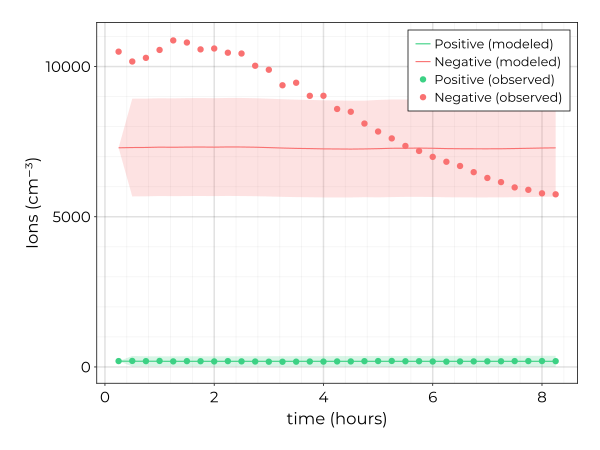
\includegraphics[width=0.85\columnwidth]{heart-chamber/assimilation/ions/ion_totals.png}
\end{figure}


Add in numbers/plots for $\mathrm{NO_3^-}$ ions from latest implementation of the mechanism.


\section{Next Steps}


- Extend mechanism to include heterogeneous (mixed phase) reaction types
- Extend mechanism to include fixed rate surface deposition
- Extend mechanism to include direct generation of $\mathrm{O_2^-}$ at some rate (learned via 4d-var) for the PCO on portions
- Incorporate the cd-EKF and continue to refine integration techniques
- Perform fixed temperature/pressure long time integration tests per the Boldi thesis.
- Update reaction rates further with recent JPL Kinetic evaluations.

%% \section{An Evaluation of Photocatalytic Ionization}



%% \begin{itemize}
%% \item sensor fusion
%% \item photolysis
%% \item docker ingestion framework
%% \item Master Chemical Mechanism
%% \item CRI Mechanism
%% \item AutoChem
%% \item data assimilation
%% \item Overview of all sensor in sensor matrix
%% \item Overview of measurement capabilities (list of species, uncertainty levels, etc...)
%% \item Overview of containerized data acquisition pipeline
%% \item NodeRed
%% \item InfluxDB
%% \item Grafana
%% \item Quarto
%% \item Automatic Alerts
%% \item Automatic Reports
%% \item MCM Implementation in Julia
%% \item Direct computation of Photolysis rates
%% \item Combination with Dr. Lary's AutoChem
%% \item Addition of Ion Chemistry from MIT Lightning disseration
%% \item Visualization of chemical cycles
%% \item SciML methods to infer below detection limits
%% \item Ion Chemistry
%% \item Indoor Air Quality
%% \item Photocatalytic Ionization
%% \end{itemize}


